% !TeX spellcheck = nl_NL

\competentie
{% competentieformulier
	\competentieformulier
	{% toelichting
		Je bent onderzoekend en brengt verschillende aspecten van een vraagstuk of probleem vanuit verschillende perspectieven in kaart. Je verzamelt relevante informatie uit erkende bronnen. Je analyseert deze informatie en brengt deze op systematische wijze met elkaar in verband. Op basis hiervan vorm je een oordeel en kom je tot een oplossing. Je kunt verschillende invalshoeken gebruiken om tot nieuwe ideeën en oplossingen te komen.
	}
	{% deelcompetenties
		analyse en oordeelsvorming,%
		onderzoeken,%
		creativiteit%
	}
	{% beroepstaken
		1...,%
		2...,%
		Etc.%
	}
	{%
		Bewijs uit stage
	}
	{%
		Deze competentie moet je verplicht aantonen tijdens het assessment. Voor onderzoekend vermogen is het met een voldoende beoordeelde onderzoeksrapport een verplicht bewijs. Naast het onderzoeksrapport mag je nog een ander bewijs selecteren: een beroepsproduct of een ervaringsverslag in de vorm van een ingevuld STARR-formulier. Het onderzoeksverslag wordt voorafgegaan door een toelichting in de vorm van een STARR-formulier. Als je nog een beroepsproduct toe voegt, wordt dit ook voorafgegaan door een toelichting in de vorm van een STARR-formulier.
	}
	{% verwijzing naar bewijs
		Onderzoeksrapport,%
		Bewijs 2%
	}
}
{% bewijzen
	\bewijs
	{% naam
		Onderzoeksrapport
	}
	{% starr
		\starr
		{% betreft
			b
		}
		{% datum
			c
		}
		{% situatie
			d
		}
		{% taak
			e
		}
		{% activiteiten
			f
		}
		{% resultaat
			g
		}
		{% reflectie
			h
		}
	}
	{% bewijs
		{%
			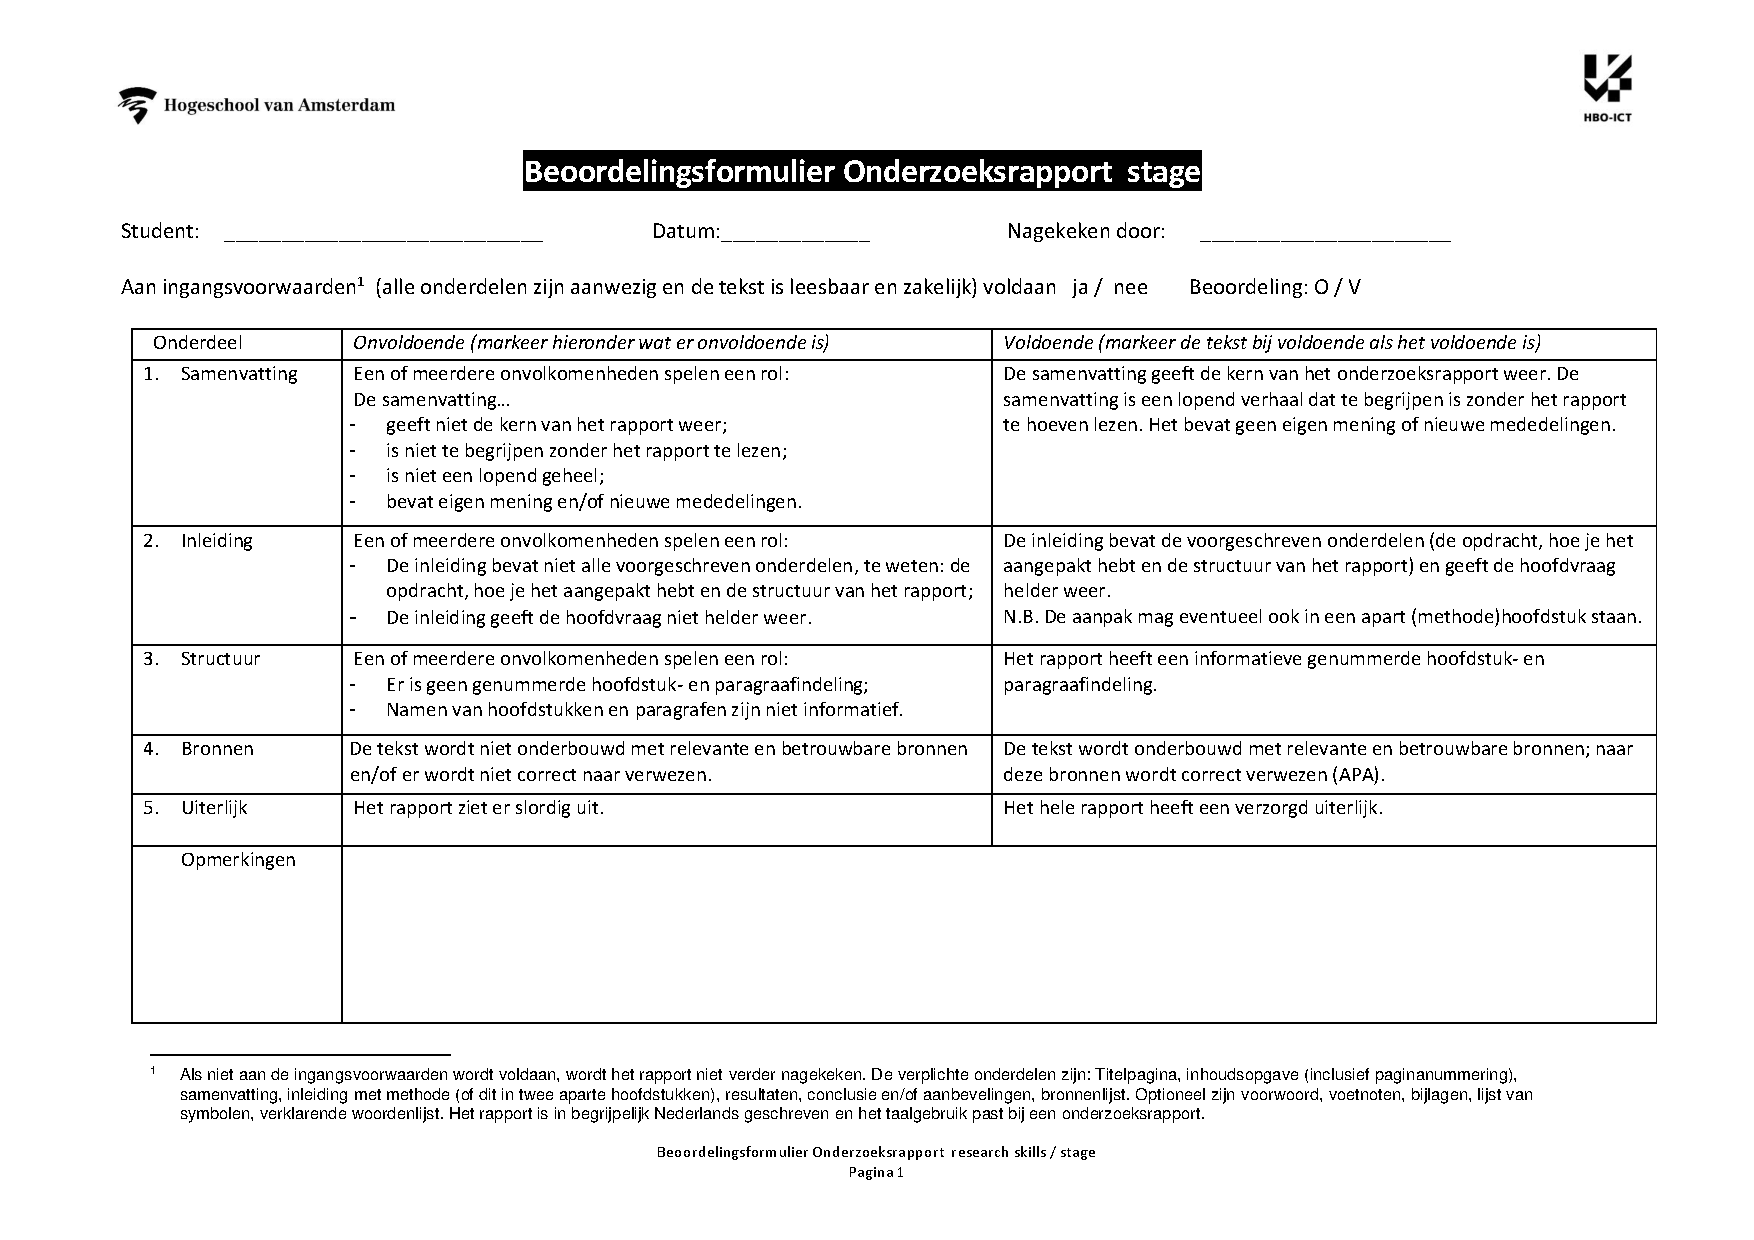
\includepdf[
				pages=1,
				frame,
				scale=0.90,
				pagecommand={
					\section*{Bewijs}
					Zie \autoref{appendix:Onderzoeksrapport} voor het onderzoeksrapport.
				}
			]{./appendices/beoordelingsformulier-onderzoeksrapport}
			
			\includepdf[
				pages=2-,
				frame,
				scale=0.90,
				pagecommand={}
			]{./appendices/beoordelingsformulier-onderzoeksrapport}
		}
	},
	\bewijs
	{% naam
		a
	}
	{% starr
		\starr
		{% betreft
			b
		}
		{% datum
			c
		}
		{% situatie
			d
		}
		{% taak
			e
		}
		{% activiteiten
			f
		}
		{% resultaat
			g
		}
		{% reflectie
			h
		}
	}
	{% bewijs
		
	}
}
